% ===========================================================================
\section{Materiais e m\'etodos}
\label{sec:metodos}
% ===========================================================================

Esta se\c{c}\~ao descreve como o trabalho foi conduzido, com detalhe suficiente para que um
terceiro possa reproduzi-lo ou contest\'a-lo. Registram-se o ambiente, o corpus de entrada, o
m\'etodo de especifica\c{c}\~ao, as decis\~oes de estrat\'egia geom\'etrica e de materiais, o
procedimento experimental e as amea\c{c}as \`a validade.

\subsection{Natureza e classifica\c{c}\~ao da pesquisa}

Quanto \`a natureza, a pesquisa \'e aplicada: n\~ao busca uma lei geral, e sim demonstrar que
um \emph{pipeline} espec\'ifico produz um artefato verific\'avel. Quanto \`a abordagem, \'e
quantitativa e qualitativa --- quantitativa na medi\c{c}\~ao de envelope, contagem de faces e
tempos de render; qualitativa na avalia\c{c}\~ao comparativa das vistas. Quanto ao objetivo,
\'e explorat\'oria com componente experimental controlado. Quanto ao procedimento, \'e um
estudo de caso \'unico, com um \'unico objeto e uma \'unica configura\c{c}\~ao de
\emph{software}.

Essa configura\c{c}\~ao tem uma consequ\^encia metodol\'ogica expl\'icita: como o estudo de
caso n\~ao permite generaliza\c{c}\~ao estat\'istica, todas as afirma\c{c}\~oes deste artigo
s\~ao \emph{sobre o caso}, e as generaliza\c{c}\~oes s\~ao apresentadas como hip\'oteses a
testar, n\~ao como conclus\~oes.

\subsection{Ambiente computacional}

O Quadro~\ref{qua:ambiente} registra as vers\~oes exatas. A fixa\c{c}\~ao das vers\~oes \'e
parte do m\'etodo, porque tanto a API do Blender quanto os nomes de par\^ametros de
configura\c{c}\~ao de render mudam entre vers\~oes.

\begin{quadro}[htbp]
\centering
\caption{Ambiente computacional e vers\~oes}
\label{qua:ambiente}
\footnotesize
\begin{tabular}{>{\raggedright\arraybackslash}p{4.4cm}>{\raggedright\arraybackslash}p{10.0cm}}
\toprule
\textbf{Componente} & \textbf{Especifica\c{c}\~ao} \\
\midrule
Sistema operacional & GNU/Linux (ambiente local de desenvolvimento) \\
Blender & 5.2.1 LTS, unidades m\'etricas, \texttt{scale\_length = 1,0} \\
Motor de render & \texttt{BLENDER\_EEVEE} com tra\c{c}ado de raios habilitado \\
API de modelagem & \texttt{bpy} e \texttt{bmesh} (Python embutido no Blender) \\
Servidor MCP & \texttt{blender-mcp} \cite{blendermcp2025}, transporte \texttt{stdio} \\
Lan\c{c}ador do servidor & \texttt{uvx} \\
Cliente MCP & agente de codifica\c{c}\~ao em ambiente de desenvolvimento (VS Code) \\
Persist\^encia & \texttt{car-lotus-elise-111s.blend} (arquivo \'unico) \\
Diagramas & \texttt{mermaid-cli} com navegador do sistema \\
Composi\c{c}\~ao do texto & \LaTeX{} (\texttt{pdflatex}) com \texttt{bibtex} \\
Depend\^encias externas & nenhuma \\
\bottomrule
\end{tabular}
\fonte{elaborado pelo autor (2026).}
\end{quadro}

A aus\^encia de depend\^encias externas \'e deliberada. Ela reduz a superf\'icie de falha,
garante que o \emph{build} n\~ao dependa de pacotes de terceiros e mant\'em o tempo de
reconstru\c{c}\~ao baixo o suficiente para permitir itera\c{c}\~oes r\'apidas ---
propriedade relevante porque, como se mostra na Se\c{c}\~ao~\ref{sec:resultados}, verificar
\'e muito mais caro que reconstruir.

\subsection{Arquitetura do \emph{pipeline} e media\c{c}\~ao por MCP}

A arquitetura tem tr\^es camadas (Figura~\ref{fig:arquitetura}). Na camada superior, um
agente de codifica\c{c}\~ao atua como cliente MCP. Na intermedi\'aria, o servidor
\texttt{blender-mcp} exp\~oe ferramentas e traduz chamadas do protocolo em c\'odigo Python.
Na inferior, o Blender executa esse c\'odigo na sess\~ao viva e devolve resultados.

A propriedade arquitetural relevante \'e que \emph{n\~ao existe caminho de edi\c{c}\~ao
manual}. Toda modifica\c{c}\~ao da cena \'e consequ\^encia da execu\c{c}\~ao de um
\emph{script}. Se um ajuste n\~ao est\'a no \emph{script}, ele n\~ao sobrevive ao
pr\'oximo \emph{build} --- e \'e essa propriedade, formulada como princ\'ipio na
constitui\c{c}\~ao do projeto, que sustenta a reprodutibilidade.

\begin{figure}[htbp]
  \centering
  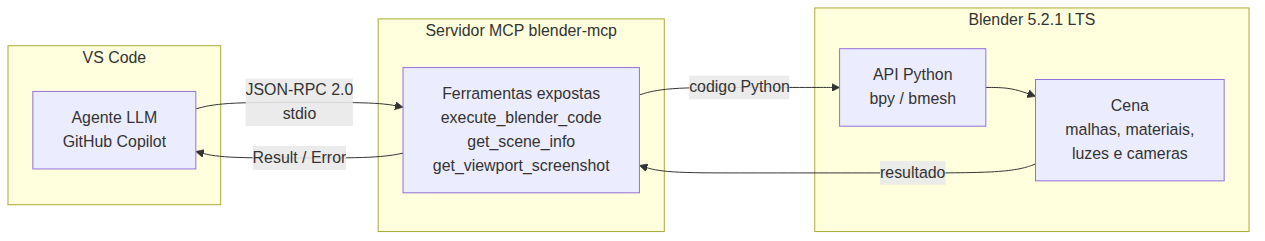
\includegraphics[width=0.92\textwidth]{figures/arquitetura-mcp.png}
  \caption{Arquitetura de tr\^es camadas. O agente (cliente MCP) n\~ao manipula a interface
           do Blender: ele invoca ferramentas cujo efeito \'e a execu\c{c}\~ao de c\'odigo.}
  \label{fig:arquitetura}
  \fonte{elaborado pelo autor (2026).}
\end{figure}

\subsection{M\'etodo de especifica\c{c}\~ao adotado}

Adota-se uma adapta\c{c}\~ao enxuta do Desenvolvimento Orientado por Especifica\c{c}\~ao,
com quatro artefatos encadeados e versionados:

\begin{enumerate}[label=\arabic*),leftmargin=1.4cm,itemsep=2pt]
  \item \textbf{Constitui\c{c}\~ao} --- princ\'ipios n\~ao negoci\'aveis: fidelidade \`a
        refer\^encia em caso de conflito com o texto; fidelidade dimensional com
        toler\^ancia de 2\,cm; qualidade de malha; reprodutibilidade por \emph{script};
        materiais fisicamente plaus\'iveis; verifica\c{c}\~ao visual documentada; e
        disciplina de mudan\c{c}a.
  \item \textbf{Especifica\c{c}\~ao} --- 21 requisitos funcionais, quatro requisitos n\~ao
        funcionais e nove crit\'erios de aceita\c{c}\~ao, cada um com m\'etodo de
        verifica\c{c}\~ao declarado.
  \item \textbf{Projeto} --- quatro registros de decis\~ao de arquitetura, dimens\~oes de
        refer\^encia e rejei\c{c}\~ao expl\'icita de alternativas.
  \item \textbf{Tarefas} --- doze tarefas com depend\^encias, condi\c{c}\~ao de conclus\~ao e
        ponto de verifica\c{c}\~ao.
\end{enumerate}

A ordem de preced\^encia em caso de conflito \'e: imagem de refer\^encia $\succ$ ficha
dimensional $\succ$ texto descritivo. Essa preced\^encia foi escolhida porque as imagens
representam o objeto real, enquanto o texto descritivo \'e uma interpreta\c{c}\~ao do objeto.
A primeira decis\~ao de arquitetura --- modelagem 100\% procedimental, sem \emph{assets}
externos --- e a segunda --- arcos de roda por modula\c{c}\~ao do perfil, sem
opera\c{c}\~oes booleanas --- condicionam todo o restante do m\'etodo.

\subsection{Corpus de refer\^encia}

O corpus de entrada \'e um conjunto de seis fotografias do ve\'iculo real, apresentado na
Figura~\ref{fig:referencias}. As imagens cobrem as vistas frontal, lateral, traseira (duas
tomadas), superior e tr\^es-quartos. Uma das imagens mostra um ve\'iculo de cor diferente
--- branco --- e foi utilizada exclusivamente para leitura de \emph{forma} (recortes,
grelhas, posi\c{c}\~ao relativa de elementos) e n\~ao para cor; essa restri\c{c}\~ao de uso
\'e registrada como premissa.

\begin{figure}[htbp]
  \centering
  \begin{tabular}{ccc}
    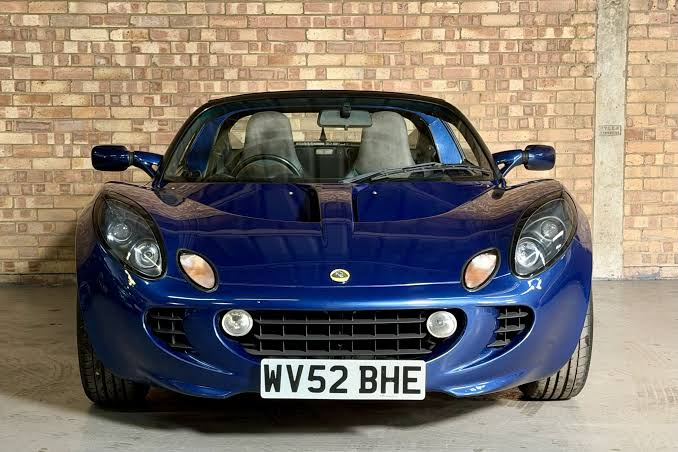
\includegraphics[width=0.29\textwidth]{figures/ref-frontal.jpeg} &
    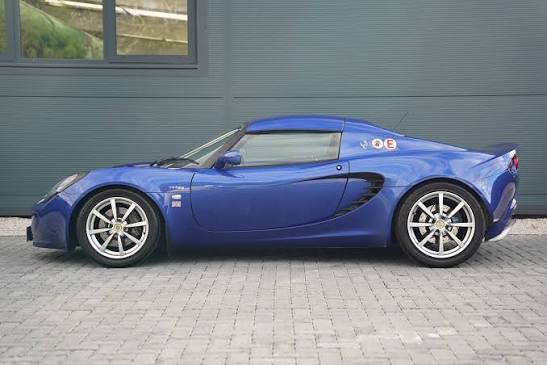
\includegraphics[width=0.29\textwidth]{figures/ref-lateral.jpeg} &
    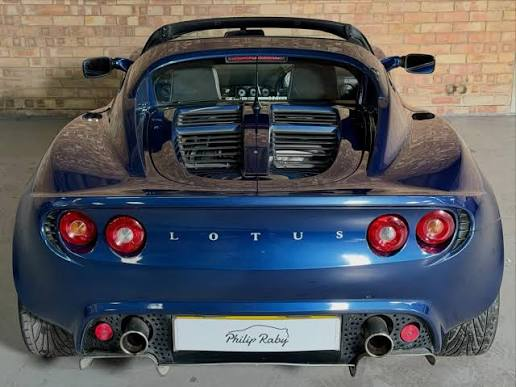
\includegraphics[width=0.29\textwidth]{figures/ref-traseira1.jpeg} \\[2pt]
    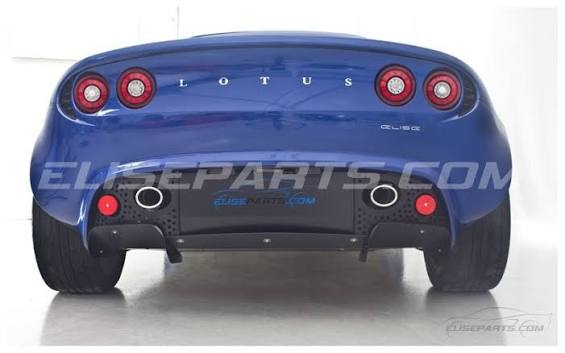
\includegraphics[width=0.29\textwidth]{figures/ref-traseira2.jpeg} &
    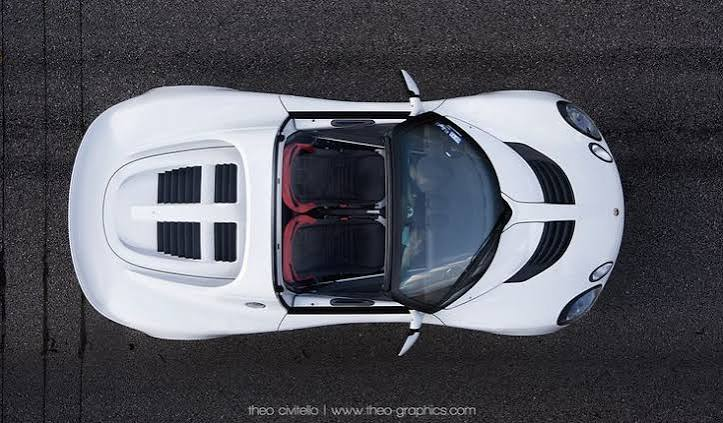
\includegraphics[width=0.29\textwidth]{figures/ref-superior.jpeg} &
    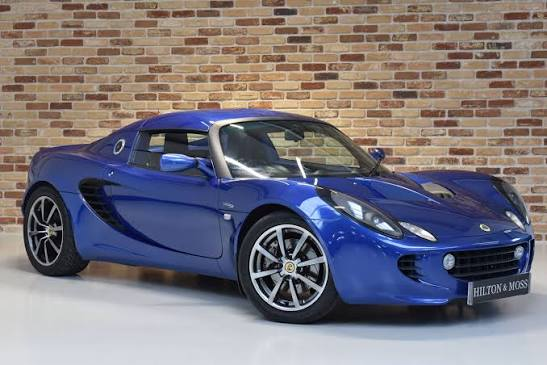
\includegraphics[width=0.29\textwidth]{figures/ref-car.jpeg}
  \end{tabular}
  \caption{Corpus de refer\^encia (\emph{ground truth} visual). Da esquerda para a direita e de
           cima para baixo: frontal, lateral, traseira, traseira em tr\^es-quartos, superior e
           tr\^es-quartos com a pintura azul.}
  \label{fig:referencias}
  \fonte{acervo do projeto (\texttt{images/}).}
\end{figure}

Duas caracter\'isticas do corpus condicionam o m\'etodo. A primeira \'e a aus\^encia de
\emph{blueprints} ortogr\'aficos: as fotografias t\^em perspectiva, o que impede a
medi\c{c}\~ao direta de propor\c{c}\~oes \cite{hartley2004}. A segunda \'e a
resolu\c{c}\~ao moderada das imagens (entre $516\times387$ e $723\times423$ pixels),
insuficiente para extrair detalhes microm\'etricos.

\subsection{Deriva\c{c}\~ao das dimens\~oes de refer\^encia}

O procedimento de deriva\c{c}\~ao seguiu tr\^es passos, na ordem de preced\^encia do
m\'etodo: (i)~\textbf{envelope como restri\c{c}\~ao dura}, adotando comprimento, largura e
altura da especifica\c{c}\~ao do cliente e de ficha p\'ublica do Series~1, com
toler\^ancia de $\pm2$\,cm; (ii)~\textbf{propor\c{c}\~oes relativas das fotografias},
estimando alturas de cintura, de \emph{deck} e de saia e a posi\c{c}\~ao relativa dos eixos
nas vistas lateral e superior, normalizadas por elementos de refer\^encia internos
(di\^ametro da roda, altura total); e (iii)~\textbf{consist\^encia com a ficha de pneus},
usando os raios derivados das designa\c{c}\~oes comerciais como verifica\c{c}\~ao cruzada.

A Tabela~\ref{tab:dimensoes} consolida os valores adotados. Cada valor \'e classificado
quanto \`a origem, permitindo que um revisor saiba quais n\'umeros s\~ao restri\c{c}\~oes
externas e quais s\~ao estimativas do autor.

\begin{table}[htbp]
\centering
\caption{Dimens\~oes de refer\^encia adotadas e origem de cada valor}
\label{tab:dimensoes}
\footnotesize
\begin{tabular}{>{\raggedright\arraybackslash}p{4.4cm}>{\raggedright\arraybackslash}p{2.6cm}>{\raggedright\arraybackslash}p{2.6cm}>{\raggedright\arraybackslash}p{4.4cm}}
\toprule
\textbf{Par\^ametro} & \textbf{Valor} & \textbf{Origem} & \textbf{Uso} \\
\midrule
Comprimento total & 3,726 m & especifica\c{c}\~ao e ficha & restri\c{c}\~ao dura \\
Largura total & 1,718 m & especifica\c{c}\~ao e ficha & restri\c{c}\~ao dura \\
Altura total & 1,117 m & especifica\c{c}\~ao e ficha & restri\c{c}\~ao dura \\
Dist\^ancia entre eixos & 2,300 m & ficha do Series 1 & restri\c{c}\~ao dura \\
Bitola dianteira & 1,419 m & ficha do Series 1 & restri\c{c}\~ao dura \\
Bitola traseira & 1,454 m & ficha do Series 1 & restri\c{c}\~ao dura \\
Pneu dianteiro 185/55R15 & raio 0,292 m & designa\c{c}\~ao comercial & derivado \\
Pneu traseiro 205/50R16 & raio 0,306 m & designa\c{c}\~ao comercial & derivado \\
Altura de cintura & $\approx$ 0,80 m & estimativa fotogr\'afica & estimativa \\
Topo do \emph{deck} do motor & $\approx$ 0,92 m & estimativa fotogr\'afica & estimativa \\
Altura m\'inima de saia & $\approx$ 0,12 m & estimativa fotogr\'afica & estimativa \\
\bottomrule
\end{tabular}
\fonte{elaborado pelo autor (2026). As estimativas fotogr\'aficas t\^em incerteza n\~ao
quantificada, conforme discutido na Se\c{c}\~ao~\ref{sec:ameacas}.}
\end{table}

\subsection{Estrat\'egia de constru\c{c}\~ao geom\'etrica}

O casco principal \'e constru\'ido como um \emph{loft} de se\c{c}\~oes transversais ao longo
do eixo longitudinal, sendo cada esta\c{c}\~ao um perfil fechado de dezesseis pontos. A
escolha por essa representa\c{c}\~ao, em vez de NURBS \cite{piegl1997}, deve-se a tr\^es
raz\~oes: a parametriza\c{c}\~ao por tabela \'e diretamente leg\'ivel e edit\'avel; a
topologia resultante \'e quadrangular por constru\c{c}\~ao; e o ajuste de uma
esta\c{c}\~ao afeta apenas uma faixa da malha, o que torna a itera\c{c}\~ao localizada e
previs\'ivel.

O recorte do arco de roda \'e obtido elevando a cota do fundo nas esta\c{c}\~oes
pr\'oximas aos eixos, produzindo um ``t\'unel'' suave sobre o pneu com a malha
quadrangular preservada. A alternativa --- diferen\c{c}a booleana entre o casco e um
cilindro --- foi rejeitada porque produz n-gons e tri\^angulos exatamente sobre a aresta
viva do para-lama, que \'e a regi\~ao de maior visibilidade do reflexo. As extremidades
(nariz e cauda) s\~ao fechadas por uma tampa que, por constru\c{c}\~ao, s\'o emite quads,
evitando o n-gon de dezesseis lados que o preenchimento ing\^enuo do contorno produziria.

Os recortes de forma --- entradas de ar laterais e alojamento dos far\'ois --- s\~ao
implementados como deslocamento de v\'ertices com fun\c{c}\~ao de atenua\c{c}\~ao, e n\~ao
como mapas de normais. A profundidade do rebaixo \'e um par\^ametro verific\'avel, e a
exist\^encia de geometria real sob a superf\'icie assegura que o sombreamento resultante
seja geom\'etrico, e n\~ao uma ilus\~ao de superf\'icie.

\subsection{Estrat\'egia de materiais}

Os materiais seguem a formula\c{c}\~ao de renderiza\c{c}\~ao fisicamente baseada
(Se\c{c}\~ao~\ref{sec:fundamentacao}), com o n\'o \emph{Principled BSDF} como bloco
central. Tr\^es decis\~oes merecem destaque.

\textbf{Pintura multicamada.} O material da carroceria combina uma cor base azul profunda
convertida de sRGB para linear, uma perturba\c{c}\~ao de alta frequ\^encia para simular os
flocos met\'alicos micro-m\'etricos e uma camada de verniz com \'indice de refra\c{c}\~ao e
rugosidade pr\'oprios. O escurecimento das bordas \'e obtido por uma rampa de cor controlada
pelo \emph{facing} de um n\'o de peso de camada.

\textbf{Convers\~ao de espa\c{c}\~o de cor.} Todas as cores s\~ao definidas em sRGB e
convertidas para o espa\c{c}\~o linear antes de serem atribu\'idas ao n\'o. A
convers\~ao incorreta \'e uma fonte comum e sutil de erro de tom, porque o resultado
\emph{parece} plaus\'ivel, mas com satura\c{c}\~ao sistematicamente deslocada
\cite{fairchild2013}.

\textbf{Transmiss\~ao.} Vidros e lentes usam transmiss\~ao com rugosidade distinta por
aplica\c{c}\~ao --- o policarbonato dos far\'ois mais pr\'oximo do especular perfeito, o
vidro do para-brisa com rugosidade ligeiramente maior \cite{walter2007}. A
refra\c{c}\~ao por tra\c{c}ado de raios precisa ser habilitada explicitamente nos
materiais transparentes para que o efeito apare\c{c}a no motor EEVEE
\cite{blender5manual}.

\subsection{Estrat\'egia de ilumina\c{c}\~ao e c\^ameras}

O \emph{rig} de ilumina\c{c}\~ao completo descrito na especifica\c{c}\~ao original
(\emph{softboxes}, \emph{light cards}, HDRI) foi declarado fora de escopo por decis\~ao do
usu\'ario. Em seu lugar adota-se um \emph{rig} neutro m\'inimo, com quatro luzes de
\'area: uma chave a aproximadamente quarenta e cinco graus, um preenchimento mais fraco do
lado oposto, uma luz de recorte traseira e um cart\~ao lateral longo. O objetivo do
\emph{rig} neutro n\~ao \'e produzir uma imagem de apresenta\c{c}\~ao, mas revelar
continuidade de superf\'icie, tornando vis\'iveis eventuais descontinuidades de curvatura.

As c\^ameras usam dist\^ancia focal longa (entre 62\,mm e 105\,mm) e ficam a dist\^ancias
entre 7,6\,m e 8,2\,m do objeto. A escolha por lentes longas minimiza a distor\c{c}\~ao de
perspectiva, aproximando a proje\c{c}\~ao de uma ortogr\'afica e facilitando a
compara\c{c}\~ao com as fotografias.

\subsection{Procedimento experimental}

O procedimento \'e composto por quatro etapas execut\'aveis por \emph{script}.

\begin{enumerate}[label=\arabic*),leftmargin=1.4cm,itemsep=2pt]
  \item \textbf{Build.} Limpeza completa da cena e reconstru\c{c}\~ao de todo o modelo,
        materiais, \emph{rig} de verifica\c{c}\~ao e c\^ameras, seguida de emiss\~ao do
        relat\'orio de malha e grava\c{c}\~ao do arquivo de cena.
  \item \textbf{Verifica\c{c}\~ao.} Render de nove vistas em baixa lat\^encia: cinco vistas
        principais, duas vistas em tr\^es-quartos, um \emph{close} de roda e duas vistas em
        material neutro (\emph{clay}) para leitura de forma sem influ\^encia da cor.
  \item \textbf{Galeria.} Render de cinco imagens de apresenta\c{c}\~ao, incluindo uma com
        \emph{rig} dram\'atico e efeito de brilho no compositor.
  \item \textbf{Compara\c{c}\~ao.} Confronto sistem\'atico entre cada render e a
        refer\^encia correspondente, com registro de aceite por crit\'erio.
\end{enumerate}

A etapa de verifica\c{c}\~ao em material neutro merece justificativa. Como a cor e o verniz
alteram a leitura da forma, uma vista em \emph{clay} remove essas vari\'aveis e permite
julgar silhueta e fluxo de arestas isoladamente. \'E o an\'alogo pr\'atico, para uma malha,
do que os mapas de zebra fazem para uma superf\'icie param\'etrica.

\subsection{Crit\'erios de aceita\c{c}\~ao}

O Quadro~\ref{qua:criterios} lista os nove crit\'erios de aceita\c{c}\~ao e o m\'etodo de
verifica\c{c}\~ao de cada um. A separa\c{c}\~ao entre verifica\c{c}\~ao num\'erica e
verifica\c{c}\~ao visual \'e expl\'icita, conforme discutido na
Se\c{c}\~ao~\ref{sec:relacionados}.

\begin{quadro}[htbp]
\centering
\caption{Crit\'erios de aceita\c{c}\~ao e m\'etodo de verifica\c{c}\~ao}
\label{qua:criterios}
\footnotesize
\begin{tabular}{>{\raggedright\arraybackslash}p{1.3cm}>{\raggedright\arraybackslash}p{6.6cm}>{\raggedright\arraybackslash}p{4.6cm}}
\toprule
\textbf{ID} & \textbf{Crit\'erio} & \textbf{M\'etodo} \\
\midrule
CA-001 & \emph{Build} reconstr\'oi o modelo sem erro & execu\c{c}\~ao do \emph{script} \\
CA-002 & Envelope dentro de $\pm2$\,cm dos alvos & medi\c{c}\~ao num\'erica \\
CA-003 & Zero n-gons e normais coerentes nos corpos & relat\'orio de malha \\
CA-004 & Silhueta lateral coerente com a refer\^encia & inspe\c{c}\~ao visual \\
CA-005 & Frente com far\'ois ovais, grelha e auxiliares & inspe\c{c}\~ao visual \\
CA-006 & Traseira com lanternas, \emph{lettering}, escapes e difusor & inspe\c{c}\~ao visual \\
CA-007 & Pintura com reflexos cont\'inuos, sem facetas & inspe\c{c}\~ao visual \\
CA-008 & Vista superior com entradas de ar, \emph{louvres} e arco de seguran\c{c}a & inspe\c{c}\~ao visual \\
CA-009 & Nomenclatura e metadados em todos os objetos & inspe\c{c}\~ao do arquivo \\
\bottomrule
\end{tabular}
\fonte{elaborado pelo autor (2026).}
\end{quadro}

\subsection{Reprodutibilidade}

A reprodu\c{c}\~ao integral do artefato exige apenas o Blender em vers\~ao compat\'ivel e o
reposit\'orio de \emph{scripts}. Os tr\^es comandos s\~ao:

\begin{lstlisting}[language=bash]
blender --background car-lotus-elise-111s.blend --python scripts/build_lotus_elise_111s.py
blender --background car-lotus-elise-111s.blend --python scripts/render_views.py
blender --background car-lotus-elise-111s.blend --python scripts/render_gallery.py
\end{lstlisting}

A execu\c{c}\~ao via MCP \'e equivalente e consiste em executar o \emph{script} dentro da
sess\~ao viva do Blender. As duas formas produzem o mesmo resultado, o que \'e verific\'avel
comparando-se o relat\'orio de malha ap\'os cada execu\c{c}\~ao. O tempo de cada etapa \'e
apresentado na Se\c{c}\~ao~\ref{sec:resultados}.

\subsection{Amea\c{c}as \`a validade}
\label{sec:ameacas}

\textbf{Aus\^encia de \emph{blueprints}.} As propor\c{c}\~oes derivam de fotografias em
perspectiva. Mesmo com normaliza\c{c}\~ao por elementos de refer\^encia internos, h\'a erro
sistem\'atico cuja magnitude n\~ao pode ser estimada sem medi\c{c}\~ao independente. Trata-se
da principal limita\c{c}\~ao de validade interna.

\textbf{Valida\c{c}\~ao pelo pr\'oprio autor.} A avalia\c{c}\~ao visual foi realizada pelo
autor do modelo. Embora renders e crit\'erio estejam registrados, n\~ao houve
avalia\c{c}\~ao cega nem m\'ultiplos avaliadores, o que impede estimar a
reprodutibilidade da avalia\c{c}\~ao.

\textbf{Cor e cadeia de imagem.} A refer\^encia fotogr\'afica passou pelo processamento da
c\^amera; o render passou pelo mapeamento de tons AgX. Diferen\c{c}as de tom entre os dois
podem decorrer da cadeia de imagem e n\~ao do material \cite{fairchild2013}.

\textbf{Ambiguidade da avalia\c{c}\~ao por imagem.} A inspe\c{c}\~ao de uma proje\c{c}\~ao
bidimensional n\~ao permite julgar com seguran\c{c}a continuidade de curvatura em
profundidade \cite{hartley2004}. A mitiga\c{c}\~ao adotada foi a verifica\c{c}\~ao
num\'erica das grandezas estruturais.

\textbf{Aus\^encia de controle experimental.} N\~ao foi executado um segundo modelo pelo
m\'etodo tradicional para servir de controle. Afirma\c{c}\~oes comparativas sobre
reprodutibilidade s\~ao, portanto, argumentativas e n\~ao experimentais.

\textbf{Depend\^encia de vers\~ao de \emph{software}.} O comportamento fotom\'etrico e a
disponibilidade de par\^ametros dependem da vers\~ao do Blender; a reprodu\c{c}\~ao em outra
vers\~ao pode exigir adapta\c{c}\~oes, discutidas na Se\c{c}\~ao~\ref{sec:desenvolvimento}.
